\chapter{Confidence Bound}
Game which have been used to test the validity of the algorithm is connect4. Connect4 is a two player game. 
So the agent have to choose one valid action depending on the board state in such way that he will win the game. This problem is similar to multi-arm bandit problem in which one has to chose arm to maximize the reward or which minimize the regret.

\section{KL-UCB}
During the self play and doing Monte Carlo Tree Search(MCTS), we are using KL-UCB to select action given the history of rewards. In multi-arm bandit problem, KL-UCB has less regret than the UCB1. We want to see whether this also work and improves the learning time of agent.

For each state and action of game we store reward during self play and the create data for agent to learn upon those examples. Moreover reward should be either 0 or 1 .\\
For a state having k valid actions
 \begin{steps}
  
  \item Choose every action once.
  \item Then choose $A_{t}$ action at t - time where $t>k$
	   
$$ A_{t} = argmax_{i}\; \max \left \lbrace x  \in \lbrack 0,1 \rbrack  : d(\hat{x}_{i}(t-1), x) <=  \dfrac{1 + (\log N)^{2}}{N_{i}} \right \rbrace  $$

$A_{t} = $ Action at time t \\
$\hat{x}_{i}  = $ Average reward of taking $i^{th}$  action in past \\
$N = $ Total number of action taken\\
$N_{i} = $ Number of times $i^{th}$ action has been taken\\



\end{steps}

\section{Baseline results}
Baseline for above algorithm is using UCB1 as it confidence bound in MCTS during self-play. The rest of the setup like Neural Network Architecture, hyperparameters remains same for both the experiments.

\section{Experiment}
Instead of using UCB1 in the action selection process during MCTS we are using KL-UCB. All other environment parameters remain same as that of Baseline. We calculate training loss and compare with the baseline. Moreover we also do tournament matches between baseline and new model for ensuring the result.

Baseline in master branch and kl-ucb on this branch.\\
\url{https://github.com/vishalkumarchaudhary/connect4/tree/kl-ucb}

\subsection{Results}

\begin{figure}
 	[!htb]\centering
    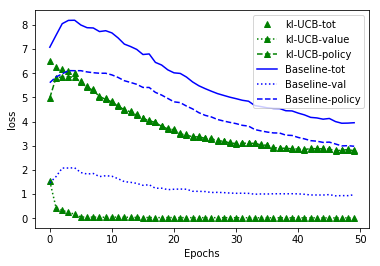
\includegraphics[width=6in]{images/kl-ucbVSbaseline.png}
    \caption{Loss function during the training of Neural Network with $KL-UCB$ confidence bound compared with UCB1 confidence bound}
  \label{fig:phase}
  \end{figure}

Moreover when the KL-UCB models had tournament with UCB1 models, 52 wins , 39 loses and 9 draws were the average roundup  results over 10 such models. This show that the new model is learning  better  than the previous model.

\clearpage
\section{Thomson sampling confidence bound}
While applying this bound with the assumption that the reward $Q(a)$ follows $Beta(\alpha,\beta)$ distribution. We have reward which are success or failures, so reward for each iteration comes from bernoulli distribution. So the posterior distribution is again $Beta$ distribution with $\alpha$ and $\beta$ parameters changed. The value of $Beta(\alpha,\beta)$ is in interval of [0,1] and $\alpha$ and $\beta$ is the count of success and failure respectively. So
$$ q_{i} \sim Beta(\alpha_{i},\beta_{i}) $$
$$ A_{t} = argmax_{i}\left \lbrace q_{i} \right \rbrace $$
$A_{t}$ is the action taken at time t, $q_{i}$ is the reward of $i^{th}$ action. So $A_{t}$ is the action which gives maximum reward after sampling from all distribution.

Some salient features of Thomspon sampling :
\begin{enumerate}
\item  Robust to delay rewards because this is randomised algorithm.
\item  Use of prior into solution can be easily incorporated and it is not possible in KL-UCB bound.
\item  Easier to implement than KL-UCB because no optimization is required other than sampling whereas in KL-UCB requires optimization and being used is Netwon-Raphson optimization.
\end{enumerate}

\section{Experiment}
Instead of using UCB1 in the action selection process during MCTS, we are using Thompson sampling method. All other environment parameters remain same as that of Baseline. We calculate training loss and compare with the baseline. Moreover we also do tournament matches between baseline and new model for ensuring the result.

This model is in Thomson-sampling branch.
\url{https://github.com/vishalkumarchaudhary/connect4/tree/thompson-sampling}

\subsection{Results}
\begin{figure}
 	[htb]\centering
    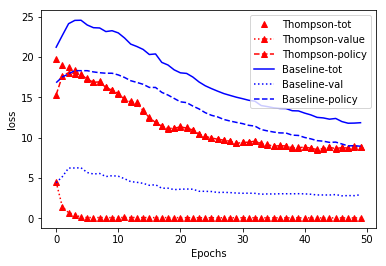
\includegraphics[width=6in]{images/thompsonVSbaseline.png}
    \caption{Comparison between Thompson and  UCB1 of training loss with respect to number of Epochs }
  \label{fig:phase}
\end{figure}


The tournament between the new model and old model remains same as that of KL-UCB model with decrease in 3 win which is very marginal and we cannot infer anything. So for this connect4 problem, Thompson sampling does as better as KL-UCB but in literature it says that it has better bounds than the KL-UCB.

\subsection{Conclusion}
Comparing the two new bounds which performs almost similar has the following loss function average over 10 experiments. These two also suggest that thier capacity of generating good examples or the exploration of probability space of rewarding action is same for connect4 game.

\begin{figure}
 	[!htb]\centering
    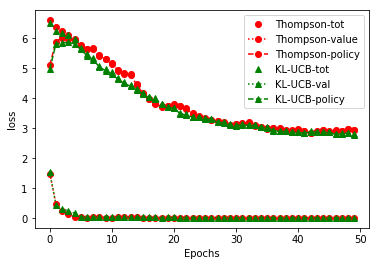
\includegraphics[width=6in]{images/kl-ucbVSthompson.png}
    \caption{Loss function during the training of Neural Network with $Thompson$ confidence bound compared with KL-UCB confidence bound}
  \label{fig:phase}
  \end{figure}
























